\usepackage{xcolor}
\usepackage{afterpage}
\usepackage{float}
\usepackage{caption}
\usepackage{tabularx}
\usepackage{pifont,mdframed}
\usepackage[bottom]{footmisc}
\usepackage{listings}
\usepackage{multicol}

\lstset{
	columns=flexible,
	basicstyle=\small\ttfamily,
	mathescape=true,
	escapeinside=||
}

\createsection{\Circuits}{Circuits}
\createsection{\InputFormat}{Input format}
\createsection{\OutputFormat}{Output format}

\renewcommand{\inputfile}{\texttt{stdin}}
\renewcommand{\outputfile}{\texttt{stdout}}
\makeatletter
\renewcommand{\this@inputfilename}{\texttt{input}}
\renewcommand{\this@outputfilename}{\texttt{output}}
\makeatother

\newenvironment{warning}
  {\par\begin{mdframed}[linewidth=2pt,linecolor=gray]%
    \begin{list}{}{\leftmargin=1cm
                   \labelwidth=\leftmargin}\item[\Large\ding{43}]}
  {\end{list}\end{mdframed}\par}
\newenvironment{danger}
{\par\begin{mdframed}[linewidth=2pt,linecolor=red!60!yellow,backgroundcolor=red!20!white]%
		\begin{list}{}{\leftmargin=1cm
				\labelwidth=\leftmargin}\item[\Large\ding{45}]}
		{\end{list}\end{mdframed}\par}

% % % % % % % % % % % % % % % % % % % % % % % % % % % % % % % % % % % % % % % % % % %
% % % % % % % % % % % % % % % % % % % % % % % % % % % % % % % % % % % % % % % % % % %

The server of the Italian Olympiads in Informatics broke right on the day of the national final contest! Will our system administrators be able to fix it before the beginning of the contest?

After a thorough analysis, it turned out that there are some fried circuits to replace. Luckily, in the laboratory of the Marconi High School there are soldering irons and enough components to rebuild the missing circuits from scratch.
Dario, our geeky tutor, has offered to build the new circuits. However, he doesn't have a design (wiring diagram) of the circuits. Help Dario design the wiring diagram of the missing circuits.

A circuit reads an array of $N$ integers through its \emph{circuit input registers} \texttt{in[$i$]} ($0 \le i < N$), and can write the result on the \emph{circuit output registers} \texttt{out[$i$]}. There are three types of circuits to replace, which have to realize the following operations.

\begin{table}[H]
	\begin{tabularx}{\textwidth}{l|X}
		\textbf{Sum} &
		Write on \texttt{out[$0$]} the sum of the $N$ input integers.\\[5pt]
		\hline \\[-10pt]
		\textbf{Prefix sum} &
		Write on the output registers the prefix sums array, defined by
		$\texttt{out[$i$]} = \texttt{in[$0$]} + \cdots + \texttt{in[$i$]}$ for $0 \le i < N$.\\[5pt]
		\hline \\[-10pt]
		\textbf{Maximum subarray} &
		Write on \texttt{out[$0$]} the largest number which can be obtained as sum of consecutive elements in the input array (i.e., which can be written as $\texttt{in[$i$]} + \cdots + \texttt{in[$j$]}$ for $0 \le i \le j < N$). The empty array is a valid subarray, so the result of this operation is always at least $0$.
	\end{tabularx}
\end{table}

Besides input and output registers, a circuit can contain \emph{intermediate registers}. Moreover, there exist \emph{special registers} which provide \emph{constants} that can be used as input to other components.

A circuit is formed of several \emph{components}, as in the example shown in Figure~1. Each component is connected to two input registers and one output register, and implements one among the following mathematical operations:
sum (\texttt{+}), difference (\texttt{-}) e maximum (\texttt{max}).
As soon as the values of both the input registers are written, the component performs the computation and, after a clock cycle, writes the result on its output register. The output register can in turn be connected to one or more components, which will perform their computation as soon as they have both their inputs available, and so on.

The circuit input registers can only be used as inputs for components, while intermediate and output registers must be outputs of \textbf{exactly one} component. The circuit computation ends when all registers have been written to.

\begin{figure}[t]%
	\centering\includegraphics[scale=1]{asy_circuiti/figs.pdf}
	\caption{Sample realization of the formula:
	\[
	\texttt{out[$0$]} = \max(\texttt{in[$0$]} + \texttt{in[$1$]} + 5 + \texttt{in[$3$]},
	(5 + \texttt{in[$3$]}) - (\texttt{in[$3$]} + \texttt{in[$4$]})) + \texttt{in[$5$]}
	\]} \label{fig}
\end{figure}

For each circut that has to be designed, you know its type (sum, prefix sum, or maximum subarray), the number $N$ of its input registers, and the desired computation time $C$ (expressed in clock cycles).

Help Dario design all the missing circuits, ensuring their correctness \textbf{for any input data}, while keeping their computation time is as close as possible to the one desired for that circuit. Try also not to use too many components: every circuit comes with $1100$ components for free, but any further component has to be paid for!

\pagebreak
The circuits you need to design are the following.
\begin{center}
	\begin{tabular}{c|c|c|c}
		\textbf{Input} & \textbf{Type} & $N$ & $C$ \\[5pt]
		\hline \\[-10pt]
		\texttt{input000.txt} & Sum & 7 & 3 \\
		\texttt{input001.txt} & Sum & 256 & 8 \\
		\texttt{input002.txt} & Sum & 1093 & 11 \\[5pt]
		\hline \\[-10pt]
		\texttt{input003.txt} & Prefix sum & 7 & 5 \\
		\texttt{input004.txt} & Prefix sum & 128 & 13 \\
		\texttt{input005.txt} & Prefix sum & 371 & 15 \\[5pt]
		\hline \\[-10pt]
		\texttt{input006.txt} & Maximum subarray & 7 & 15 \\
		\texttt{input007.txt} & Maximum subarray & 64 & 31 \\
		\texttt{input008.txt} & Maximum subarray & 110 & 35 \\
		\texttt{input009.txt} & Maximum subarray & 124 & 35 \\
	\end{tabular}
\end{center}

% % % % % % % % % % % % % % % % % % % % % % % % % % % % % % % % % % % % % % % % % % %
% % % % % % % % % % % % % % % % % % % % % % % % % % % % % % % % % % % % % % % % % % %

\InputFormat

The circuits you need to design are described in the input files according to the table above. Every file contains the three integers $T$, $N$ and $C$, where $T$ represents the type of circuit to realize ($1$ for sum, $2$ for prefix sum, $3$ for maximum subarray).

% % % % % % % % % % % % % % % % % % % % % % % % % % % % % % % % % % % % % % % % % % %
% % % % % % % % % % % % % % % % % % % % % % % % % % % % % % % % % % % % % % % % % % %

\OutputFormat

The circuit you will design has to be described through its components and their connections. Each line of the output represents a component, following one of the three possible formats:
\[
C[k] = A[i]\ \texttt{op}\ B[j] \qquad C[k] = i\ \texttt{op}\ B[j] \qquad C[k] = A[i]\ \texttt{op}\ j
\]
where:
\begin{itemize}
	\item $A$, $B$ and $C$ are array names. These names must contain at most 50 alphanumeric characters (lower or upper case), and must not start with a digit.
	\item $i$, $j$, $k$ are positive integer constants, which must fit in a signed 32-bit integer.
	\item \texttt{op} is an operator at choice among \texttt{+}, \texttt{-} or \texttt{max}.
\end{itemize}
Such a line defines a component which has $A[i]$ and $B[j]$ as input registers (or the constants $i$ and $j$ respectively), $C[k]$ as output register, and implements the operation \texttt{op}.

The two special arrays \texttt{in} and \texttt{out} indicate respectively the input and output registers. It is possible to use other arrays as intermediate registers, as desired. However, before defining a component which uses a specific intermediate register as input, another component must have \textbf{previously defined} in your file that uses the same register as output.

% % % % % % % % % % % % % % % % % % % % % % % % % % % % % % % % % % % % % % % % % % %
% % % % % % % % % % % % % % % % % % % % % % % % % % % % % % % % % % % % % % % % % % %


\Scoring

The output files will be evaluated by a checker which will verify the correctness of their format and of their described circuit. It will assign to each file a score from $0$ to $10$.

If the file is not correct, it will get a score of $0$. Otherwise, it will receive a score $P$ according to the following formula:
\[
	P = 10 \cdot \min \left\{1, \frac{C_\text{desired}}{C_\text{attained}}\right\} \cdot \min \left\{1, \frac{1100}{S_\text{attained}}\right\}
\]
where $C_\text{attained}$ is the computation time of your circuit, and $S_\text{attained}$ is the number of its components. Notice that your file will get full score $10$ if and only if $C_\text{attained}$ is less or equal to $C_\text{desired}$ and $S_\text{attained}$ is less or equal to $1100$.

% % % % % % % % % % % % % % % % % % % % % % % % % % % % % % % % % % % % % % % % % % %
% % % % % % % % % % % % % % % % % % % % % % % % % % % % % % % % % % % % % % % % % % %


\Examples

The diagram shown in the statement corresponds to the following output file:
\begin{lstlisting}
add[0] = in[0] + in[1]
add[1] = 5 + in[3]
add[2] = in[3] + in[4]
add[3] = add[0] + add[1]
add[4] = add[1] - add[2]
m[7] = add[3] max add[4]
out[0] = m[7] + in[5]
\end{lstlisting}
although it is \emph{not} a correct solution for any possible input. The visualization of this output, \textbf{or any other output you produce}, can be obtained through the scripts \verb|visualizer.sh| and \verb|visualizer.py|. The latter script receives an output file through standard input and produces an \emph{Asymptote} file in standard output; this file can then be compiled through \verb|asy -f pdf <file>|. The former script automatizes this process but may not work for your system. The resulting PDF will contain a representation of the circuit, or of any errors possibly present in the file. The visualizer will place the components which trigger at the same clock cycle $t$ on the same line, in the order they are listed in the file (from left to right).

Possible input and solutions, different from the ones you have to design, are shown below.
\begin{example}
\exmpfile{circuiti.input0.txt}{circuiti.output0.txt}%
\exmpfile{circuiti.input1.txt}{circuiti.output1.txt}%
\exmpfile{circuiti.input2.txt}{circuiti.output2.txt}%
\end{example}

% % % % % % % % % % % % % % % % % % % % % % % % % % % % % % % % % % % % % % % % % % %
% % % % % % % % % % % % % % % % % % % % % % % % % % % % % % % % % % % % % % % % % % %


\Explanation

In the \textbf{first sample case}, you need to sum $3$ input integers. If the input registers are $\texttt{in[0]} = -10$, $\texttt{in[1]} = 3$, $\texttt{in[2]} = 5$, then the value of \texttt{temp[0]} will be $-7$ and the value of \texttt{out[0]} will be $-2$. The two operations must be executed one after the other, taking two clock cycles to output the result.
\begin{center}
	\vspace{-5pt}
	\includegraphics[scale=1]{asy_circuiti/fig0.pdf}
	\vspace{-5pt}
\end{center}
In the \textbf{second sample case}, given the same input registers of the previous example, the output will be: $\texttt{out[0]} = -10$, $\texttt{out[1]} = -7$, $\texttt{out[2]} = -2$. Notice that the third component has to wait the result of the second, so that the total computation time is $2$ clock cycles.
\begin{center}
	\vspace{-5pt}
	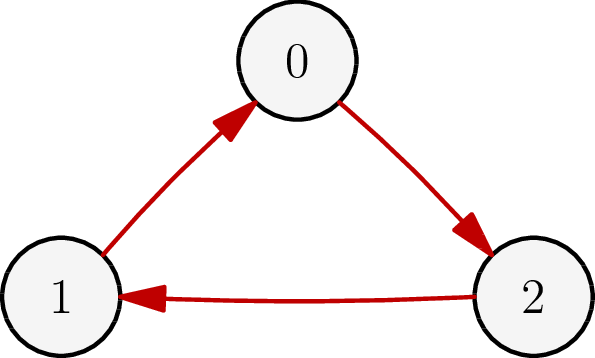
\includegraphics[scale=1]{asy_circuiti/fig1.pdf}
	\vspace{-5pt}
\end{center}
In the \textbf{third sample case}, given the same input, the value of the registers will be:
\begin{multicols}{3}
	$\texttt{somma[0]} = 0$ \\
	$\texttt{somma[12]} = -7$ \\
	$\texttt{somma[23]} = 8$ \\
	$\texttt{somma[123]} = -2$ \\
	$\texttt{mx[0]} = 0$ \\
	$\texttt{mx[1]} = 3$ \\
	$\texttt{mx[2]} = 5$ \\
	$\texttt{mx[3]} = 5$ \\
	$\texttt{mx[4]} = 8$ \\
	$\texttt{out[0]} = 8$ \\
\end{multicols}
\begin{center}
	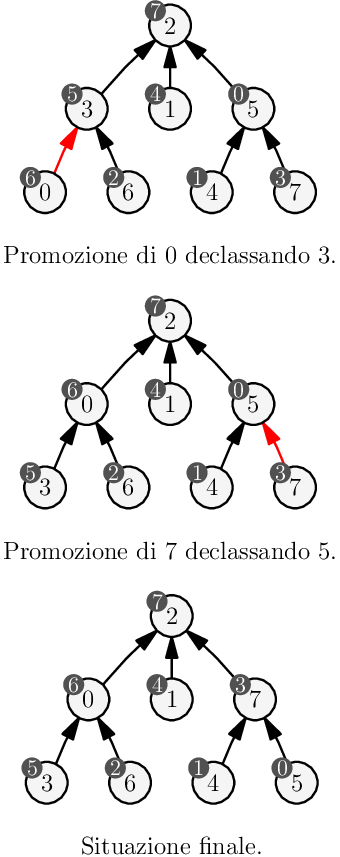
\includegraphics[scale=1]{asy_circuiti/fig2.pdf}
\end{center}
